% % -*- coding:utf-8 -*-
\documentclass[aspectratio=169,10pt]{beamer}
\nonstopmode

%\documentclass[handout,aspectratio=169,10pt]{beamer}
%\usepackage{pgfpages}
%\pgfpagesuselayout{2 on 1}[a4paper,border shrink=5mm]

\usepackage{appendixnumberbeamer}
\setbeamertemplate{footline}[frame number]
\usepackage{graphicx}
\usepackage{tikz}
\usepackage{url}
%\usepackage{mathrsfs} 
%\usepackage{unicode-math} 
%\setmathfont{XITS Math}
% color palette
\definecolor{tu01}{HTML}{84B818}
\definecolor{tu02}{HTML}{D18B12}
\definecolor{tu03}{HTML}{1BB5B5}
\definecolor{tu04}{HTML}{F85A3E}
\definecolor{tu05}{HTML}{4B6CFC}
\definecolor{tu06}{HTML}{E3B505}
\definecolor{tu07}{HTML}{AF331D}
\definecolor{tu08}{HTML}{000000}
\definecolor{tu09}{HTML}{AAAAAA}
\definecolor{tu10}{HTML}{444444}
\definecolor{tu11}{HTML}{84B818}

% mixed and light colors
\colorlet{tu01light}{tu01!33}
\colorlet{tu02light}{tu02!33}
\colorlet{tu03light}{tu03!33}
\colorlet{tu04light}{tu04!33}
\colorlet{tu05light}{tu05!33}
\colorlet{tu06light}{tu06!33}
\colorlet{tu07light}{tu07!33}
\colorlet{tu08light}{tu08!33}
\colorlet{tu09light}{tu09!33}
\colorlet{tu10light}{tu10!33}
\colorlet{tu11light}{tu11!33}

\colorlet{tu01midlight}{tu01!50}
\colorlet{tu02midlight}{tu02!50}
\colorlet{tu03midlight}{tu03!50}
\colorlet{tu04midlight}{tu04!50}
\colorlet{tu05midlight}{tu05!50}
\colorlet{tu06midlight}{tu06!50}
\colorlet{tu07midlight}{tu07!50}
\colorlet{tu08midlight}{tu08!50}
\colorlet{tu09midlight}{tu09!50}
\colorlet{tu10midlight}{tu10!50}
\colorlet{tu11midlight}{tu11!50}

\colorlet{tu01dark}{tu01!80!black}
\colorlet{tu02dark}{tu02!80!black}
\colorlet{tu03dark}{tu03!80!black}
\colorlet{tu04dark}{tu04!80!black}
\colorlet{tu05dark}{tu05!80!black}
\colorlet{tu06dark}{tu06!80!black}
\colorlet{tu07dark}{tu07!80!black}
\colorlet{tu08dark}{tu08!80!black}
\colorlet{tu09dark}{tu09!80!black}
\colorlet{tu10dark}{tu10!80!black}
\colorlet{tu11dark}{tu11!80!black}

\colorlet{lightgray}{gray!25}
\colorlet{midlightgray}{gray!50}
\colorlet{anthracite}{black!85}

% aliases
\colorlet{tudo}{tu01}
\colorlet{tuorange}{tu02}
\colorlet{tudolight}{tu01light}

% math
\definecolor{data}{RGB}{230, 128, 3}
\definecolor{functions}{RGB}{47, 50, 204}
\definecolor{params}{RGB}{64, 179, 53}
\definecolor{paramsigma}{RGB}{179, 179, 7}

\newcommand{\smally}{{\color{data}y}}
\newcommand{\bigy}{{\color{data}Y}}
\newcommand{\smallx}{{\color{data}x}}
\newcommand{\boldx}{{\color{data}\textbf{x}}}
\newcommand{\boldy}{{\color{data}\textbf{y}}}
\newcommand{\bigx}{{\color{data}\textbf{X}}}
\newcommand{\trainset}{{\color{data}\mathcal{D}}}
\newcommand{\predy}{{\color{data}\hat{y}}}
\newcommand{\basisF}{{\color{data}\Phi}}
\newcommand{\classset}{{\color{data}\mathcal{C}}}
\newcommand{\aclass}{{\color{data}c}}

\newcommand{\paramw}{{\color{params}w}}
\newcommand{\paramW}{{\color{params}\textbf{w}}}
\newcommand{\estimw}{{\color{params}\hat{w}}}
\newcommand{\estimW}{{\color{params}\hat{\textbf{w}}}}
\newcommand{\estsigma}{{\color{paramsigma}\sigma}}
\newcommand{\estSigma}{{\color{paramsigma}\hat{\sigma}}}

\newcommand{\func}{{\color{functions}f}}
\newcommand{\funcg}{{\color{functions}g}}
\newcommand{\basisf}{{\color{functions}\phi}}


\newcommand{\argmax}[1]{\underset{#1}{\operatorname{arg}\,\operatorname{max}}\;}
\newcommand{\argmin}[1]{\underset{#1}{\operatorname{arg}\,\operatorname{min}}\;}


% \usepackage{beamerthememetropolis}
\usetheme[progressbar=frametitle]{metropolis}
\newcommand{\themename}{\textbf{\textsc{metropolis}}\xspace}


\usepackage{xcolor}


\title{Machine Learning and Intelligent Systems}
\subtitle{Supervised Learning}
\author{Maria A. Zuluaga}

\institute{EURECOM - Data Science Department}
\titlegraphic{\hfill
\includegraphics[height=15mm]{images/logo_eurecom.jpg}}

\date{October 4 2022}

\begin{document}

\maketitle
\begin{frame}{Table of contents}
	\tableofcontents
\end{frame}
%TODO Table of contents
%\item Tutorial for Beamer \url{https://www.overleaf.com/learn/latex/Beamer_Presentations:_A_Tutorial_for_Beginners_(Part_1)%E2%80%94Getting_Started}
%	\item Quelle Template: \url{https://github.com/matze/mtheme}
%	\item Quelle Bild: \url{https://unsplash.com/photos/52gEprMkp7M}



\section{Setup}
\begin{frame}{Machine Learning: Definition}
	
	A computer program is said to learn from experience $E$ with respect to some class of tasks $T$ and performance measure $P$ if its performance at tasks in $T$, as measured by $P$, improves with experience $E$ (Tom M. Mitchell).
	
	\vspace{0.8cm}
	\pause
	\begin{alertblock}{Goal}
		Starting from Tom Mitchell's definition, we will formalize the supervised learning setup
	\end{alertblock}
			
\end{frame}


\subsection{The Learning Process}
\begin{frame}{Supervised Learning: Procedure}
	\centering
	 \textbf{Condensed View of Supervised Learning:}\\
	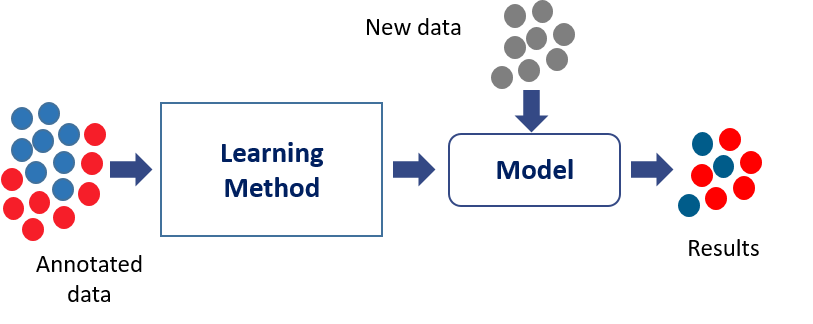
\includegraphics[width=0.5\linewidth, clip]{images/supervised}\\

	\pause
	\vspace{0.1cm}
	\textbf{Decompressed View:}\\
	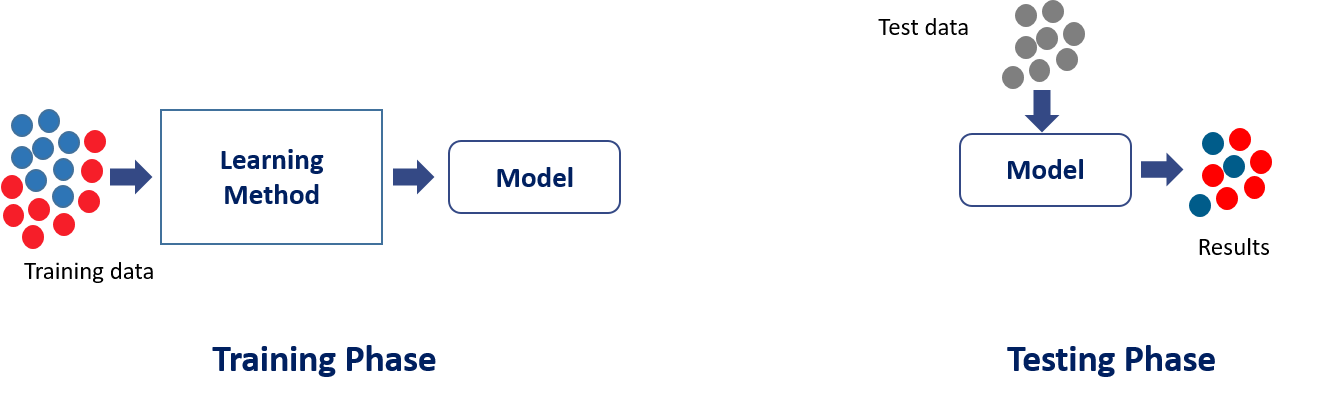
\includegraphics[width=0.8\linewidth, clip]{images/train_test}\\


\end{frame}

\subsection{Training Data}
\begin{frame}{Training Data}
	The training data comes in input pairs $(\boldx, \smally)$, with  $\boldx \in \mathbb{R}^{D}$ and $\smally \in \mathcal{C}$.\\
		\vspace{0.5cm}
	The entire training set is denoted as:
	\begin{equation*}
		\trainset = \lbrace(\boldx_{i},\smally_{i})\rbrace_{i=1}^N \,\, \subseteq \,\, \mathbb{R}^{D} \times \mathcal{C}
	\end{equation*}	

	with
	\begin{itemize}
		\item $\mathbb{R}^{D}$ - $D$-dimensional feature space
		\item $\mathcal{C}$ - label space
		\item $\boldx_{i}$ - input vector of the $i^{th}$ training sample
		\item $\smally_i$ - label of the $i^{th}$ training sample
		\item $N$ - number of training samples
	\end{itemize} 

\vspace{1.0cm}
	\alert{Question:} In the previous slide, what is $\boldx$? and $\smally$? 

\end{frame}

%\begin{frame}{Setup: Training Data}
%
%\pause
%
%	The data points $(\boldx_{i},\smally_{i})$ are drawn from an unknown probability distribution $\mathcal{P}(\bigX,\bigy)$.
%\end{frame}

\begin{frame}{Training Data}
	The \textbf{training set} points $(\boldx_{i},\smally_{i})$ are drawn from an unknown probability distribution $\mathcal{P}(\bigX,\bigy)$.
	\vspace{0.5cm}
	\pause
	\begin{alertblock}{Goal of Supervised Learning:}
		Use $\trainset$ to learn a function $\hypothesis$, such that for an \textbf{unseen point} $(\boldx,\smally) \sim \mathcal{P}$:
		\begin{equation*}
			\hypothesis(\boldx) \approx \smally
		\end{equation*}
		with  high probability
	\end{alertblock}
	\vspace{0.5cm}
	\pause
	\begin{alertblock}{Goal of this course (75\%):}
		To present different methods to obtain $\hypothesis$
	\end{alertblock}	
\end{frame}	


%	\begin{columns}
%	\column{0.5\textwidth}
%	\begin{center}

%	\end{center}
%	
%	
%	\column{0.5\textwidth}
%	\begin{center}
%		{$\smally$}\\
%		Output\\
%		Target\\
%		Label\\
%		Dependent variable\\
%	\end{center}
%\end{columns}

\begin{frame}[t]{The Output Space $\mathcal{C}$}
	\begin{itemize}
		\item $\smally \in \mathcal{C}$: Output, Target, Label, Dependent Variable.
		\item The output or label space $\mathcal{C}$ can take different forms. 
		\item Depending on this, we use a specific term to refer to the supervised learning task
	\end{itemize}

	\vspace{0.5cm}
	\begin{columns}[t]
		\column{0.02\linewidth}
		\pause
		\column{0.33\linewidth}
		\textbf{Binary Classification}\\
		$\mathcal{C} = \lbrace 0, 1 \rbrace $ or \\
		$\mathcal{C} = \lbrace -1, +1 \rbrace $
		
		\pause
		\vspace{0.7cm}
		\alert{\textbf{Example:}} 1) Red/blue ball labeling - red (1/$+$1), blue (0/$-1$)\\
		\pause
		2) Spam filtering (how?)
	
		\pause
		\column{0.33\linewidth}
		\textbf{Multi-class Classification}\\
		$\mathcal{C} = \lbrace 1, 2, \ldots, K \rbrace$ with \\
		$K \geq 2$
		
		\vspace{0.7cm}
		\alert{\textbf{Example:}} Fruit classification from photos\\
		(how?)
		\pause
		\column{0.33\linewidth}
		\textbf{Regression}\\
		$\mathcal{C} = \mathbb{R}^O$ \\
		In this course, $O=1$
		
		\vspace{0.7cm}
		\alert{\textbf{Example:}} Predict MALIS grades ($O=1$) \\
		\pause
		Predict weight and height of a person ($O=2$)
	\end{columns}
\end{frame}

\begin{frame}{The Feature Space}
	The feature vector $\boldx_i$ is a \textbf{$D$-dimensional vector} containing $D$ attributes (or features)  describing the $i^{th}$ sample. \\
		
		\vspace{1cm}
	Often {$\boldx$} is referred to as:
	\begin{itemize}
		\item Input
		\item Feature vector
		\item Attributes
		\item Independent variable
	\end{itemize}
\end{frame}			
	

\begin{frame}{The Feature Space: Examples}	

	\begin{description}
		\item[MALIS students data.] $\boldx_i = (\smallx_i^{1}, \smallx_i^{2}, \smallx_i^{3})$, with $\smallx_i^{1}$ encoding the gender ($\smallx_i^{1}$=0 or 1), $\smallx_i^{2}$ the height (cm) and $\smallx_i^{2}$ the age (years). Here $D=3$.\\
	 It is a \textbf{dense} vector, since the number of non-zero coordinates in $\boldx \gg D$.
	 \pause
	 \vspace{0.4cm}
	 \item[Text document.] The bag-of-words encoding counts the occurrences of a dictionary word in a text. Hence, in $\boldx_i = (\smallx_i^{1}, \smallx_i^{2}, \ldots \smallx_i^{D})$, $\smallx_i^{\alpha}$ is the count for the $\alpha^{th}$ word.\\
	 Most entries will have zeros. It is a \textbf{sparse} feature vector.
	 \pause
	 \vspace{0.4cm}
	 \item[Medical image.] The features represent the gray scale pixel values $\boldx_i = (\smallx_i^{1}, \smallx_i^{2}, \ldots \smallx_i^{D})$. Here, $D$ represents the total number of pixels.\\
	 \alert{Question:} Is this a sparse or a dense feature vector? 
	\end{description}
\end{frame}

\begin{frame}{Summary: Notation}
	
	\begin{table}
		\begin{tabular}{|l | l | }
			\hline
			Symbol & Reads as \\
			\hline \hline
			$\bigX$ & Input variable $(\mathbb{R}^D)$ \\ 
			$\boldx_i$ & $i^{th}$ feature vector.  Observed value of $\bigX$.  \\
			$\mathbf{\bigx}=(\boldx_1,\boldx_2, \ldots, \boldx_N)^T$ & Matrix of $N$ input $D-$dimensional vectors $\boldx_i$\\
			$\smallx_{j}$ & $j^{th}$ element of the $i^{th}$ input vector $\boldx_i$, i.e. $\smallx_i^j$ \\ 
			$\bigy$ & Output variable  $(\mathcal{C})$\\ 
			$\smally_i$ & $i^{th}$ output label\\ 
			$\boldy=(\smally_1, \ldots, \smally_N)^T$ & Observed vector of outputs $\smally_i$\\
			\hline
		\end{tabular}
		\caption{Different notation for the input and output variables}
	\end{table}
	\begin{alertblock}{Note}
		For regression, we will deal with $\smally \in \mathcal{C} =\mathbb{R}^{O=1}$
	\end{alertblock}
\end{frame}

\begin{frame}{Setup: Where are we?}
	\centering
		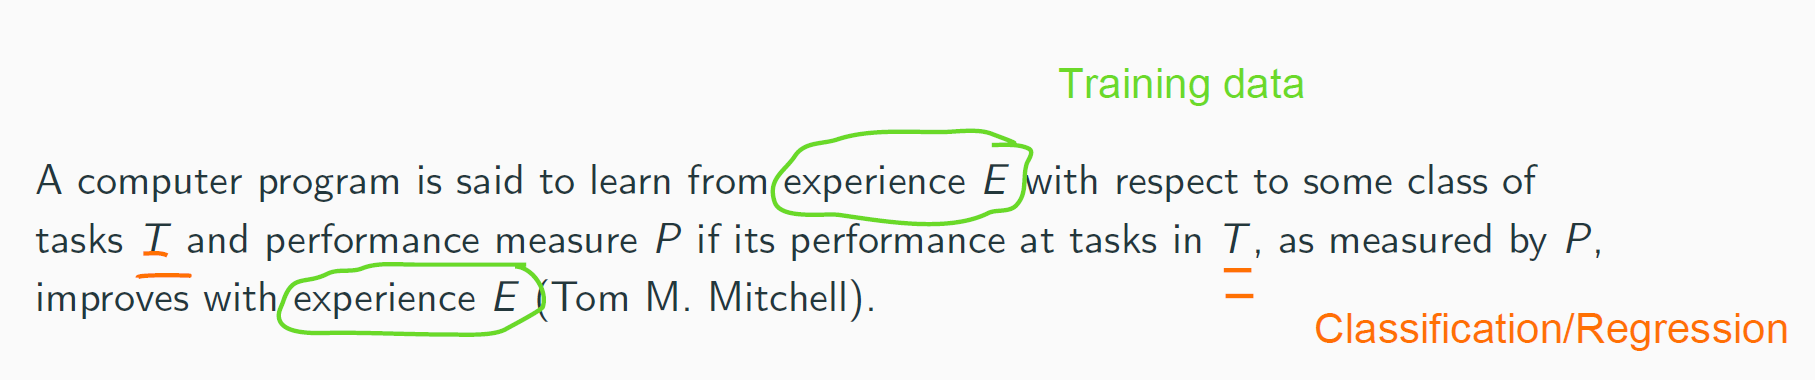
\includegraphics[width=\textwidth, clip]{images/setup_1}
\end{frame}

\subsection{The Hypothesis}
\begin{frame}{The Hypothesis Class}
	\alert{\textbf{Recall:}} The goal of supervised learning is to use $\trainset$ to learn a function $\hypothesis: \mathbb{R}^D \rightarrow \mathcal{C}$ that can predict $\smally$ from $\boldx$. \\
	\begin{center}
		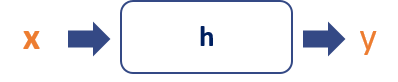
\includegraphics[width=0.4\linewidth, clip]{images/hypothesis}
	\end{center}
\pause
	\alert{\textbf{Example:}}  
	\begin{columns}
		\begin{column}[c]{0.45\paperwidth}
			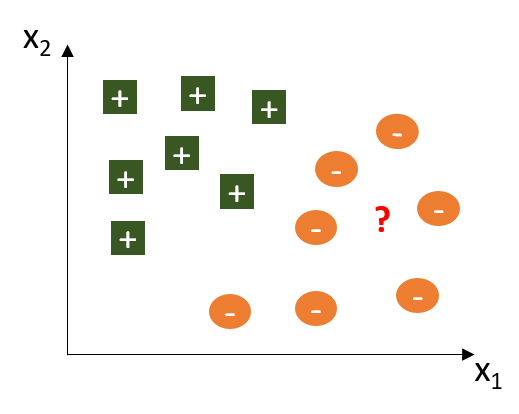
\includegraphics[width=0.7\linewidth, clip]{images/example_hypothesis}	
		\end{column}
	
	\begin{column}{0.45\paperwidth}
		\begin{itemize}
			\item $D$=
			\pause
			\item $\hypothesis(\boldx) = +1$
			\item Is this a hypothesis?
			\pause
			\item Is this a good hypothesis? 
		\end{itemize}
	\end{column}

\end{columns}
\end{frame}	

\begin{frame}{The Hypothesis Class}
	\begin{itemize}
		\item We have $\hypothesis \in \mathcal{H}$, where $\mathcal{H}$ denotes the hypothesis class
		\item \alert{\textbf{Examples:}}
		\begin{itemize}
			\item Linear Classifiers
			\item Decision Trees
			\item Neural Networks
			\item Support Vector Machines
		\end{itemize} 
	\vspace{0.4cm}
		\item First task: Pick a hypothesis class
		\item \alert{Warning:} No Free Lunch Theorem
	\end{itemize}

\end{frame}

\begin{frame}{No Free Lunch}
	\begin{columns}
		\begin{column}{0.6\linewidth}
			\begin{itemize}
				\item Which hypothesis class $\mathcal{H}$ to choose?
				\item Every ML algorithm has to make assumptions
				\item The choice will depend on the data
				\item $\mathcal{H}$ encodes assumptions about the data and its distribution
			
			\end{itemize}
		\end{column}
	\begin{column}{0.4\linewidth}
		\centering
		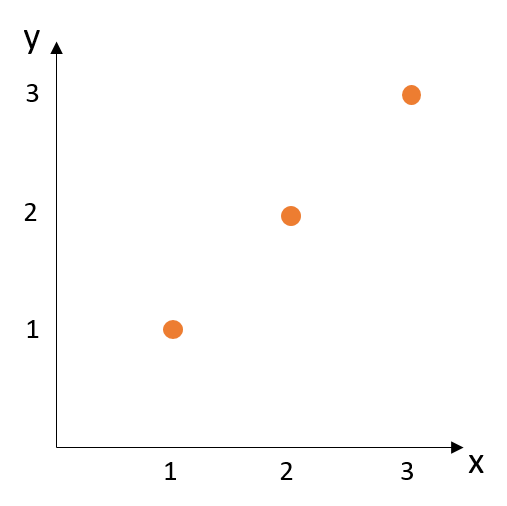
\includegraphics[width=0.8\linewidth, clip]{images/no_free}
		$\hypothesis(2.5)$=?
	\end{column}
	\end{columns}
\vspace{0.4cm}
\centering
	\textbf{No Free Lunch:} There is no single perfect choice for all problems
\end{frame}

\subsection{The Loss Function}
\begin{frame}{The Loss Function}
	\begin{itemize}
		\item \textbf{First task:} Pick a hypothesis class $\mathcal{H}$, i.e. pick a type of machine learning algorithm.
		\pause
		\item \textbf{Second task:} Find the best function within the hypothesis class,  $\hypothesis \in \mathcal{H}$.
		\pause
		\item Finding the best $\hypothesis \in \mathcal{H}$ using $\trainset$ is denoted the \textbf{learning process}.
	\vspace{0.3cm}
		\begin{center} 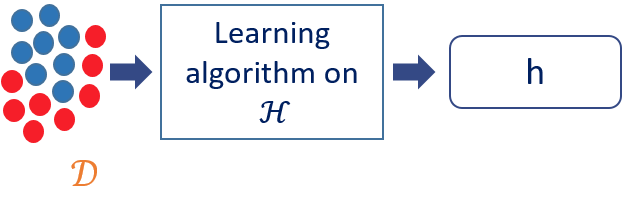
\includegraphics[width=0.5\textwidth, clip]{images/learning} \\
			\pause
		\large	\textbf{How?} 
		\end{center} 
		\vspace{0.3cm}
		\pause
		\item \textbf{Idea:} Pick $\hypothesis \in \mathcal{H}$ making the least mistakes in $\trainset$ and, preferably, the simplest.
		\pause
		\item \textbf{Measure:} Loss function
	\end{itemize}

		
\end{frame}

\begin{frame}{The Loss Function}
	\begin{itemize}
		\item A loss or risk function $\textit{l}: \mathbb{R} \rightarrow \mathbb{R}$ quantifies how well $\hypothesis(\boldx)$ approximates $\smally$.
		\begin{equation*}
			\mathit{l}(a,b)
		\end{equation*}
	\vspace{-15pt}
	\pause
	\item The lower the value of $\mathit{l}(\smally,\hypothesis(\boldx))$ the better the approximation
	\item $\mathit{l}(\smally,\smally) = 0$
	\item Typically (but not always) $\mathit{l}(\smally,\hypothesis(\boldx)) \geq 0$ for all $\smally,\hypothesis(\boldx)$
\end{itemize}
\begin{table}
\pause
\begin{tabular}{|l | c | l |}
	\hline
	\multicolumn{1}{|c|}{\textbf{Loss}} & \multicolumn{1}{c|}{\textbf{Expression}} &  \multicolumn{1}{c|}{\textbf{Task}}\\
	\hline
	0/1 Loss & $\textit{l}(\smally, \hypothesis(\boldx)) = \begin{cases} 1 & if  \hypothesis(\boldx) \neq \smally \\ 0 & \text{otherwise} \end{cases}$ & Classification\\
	Quadratic loss &	$\mathit{l}(\smally,\hypothesis(\boldx))=\left(\smally - \hypothesis(\boldx)\right)^2$ & Regression\\
	Absolute loss &	$\mathit{l}(\smally,\hypothesis(\boldx))= |\smally - \hypothesis(\boldx)|$ & Regression\\
	\hline
\end{tabular}
\caption{Common loss functions}
\end{table}

\end{frame}

\begin{frame}{Loss Minimization}
	\begin{itemize}
		\item Using the training data $\trainset$, we can compute the average loss over all the data points
		\begin{equation*}
			\mathcal{L}=\dfrac{1}{N}\sum_{i=1}^N \mathit{l}(\smally_i, \hypothesis(\boldx_i))
		\end{equation*}
		\pause
	\item Finding the best hypothesis means finding the $\hypothesis$ that minimizes the loss.
	\item This can be formalized as
	\begin{equation*}
		\hypothesis^* = \argmin{\hypothesis \in \mathcal{H}} \dfrac{1}{N}\sum_{i=1}^N \mathit{l}(\smally_i, \hypothesis(\boldx_i))
	\end{equation*}
	\end{itemize}
	
\end{frame}

\subsection{Generalization}
\begin{frame}{Generalization}
	Suppose the following hypothesis:
	\begin{equation*}
		\hypothesis(\boldx) = \begin{cases} \smally_i & \text{if} \,\, \exists \, (\boldx_{i},\smally_{i}) \in \trainset \,\,\text{s.t.} \boldx = \boldx_{i} \\
			0 & \text{otherwise} \\
		\end{cases}
	\end{equation*}
	\pause
	\alert{\textbf{Questions:}}
	\begin{itemize}
		\item What is the value of the loss $\mathcal{L}$? Pick the loss you prefer.
		\pause
		\item When new samples arrive $\boldx \notin \trainset$, how will $\hypothesis(\cdot)$ perform?
	\end{itemize}
	\vspace{0.4cm}
	When $\hypothesis(\cdot)$ has a very low loss, but it does not perform well in unseen data, we say there is \textbf{overfitting} causing that our model does not \textbf{generalize} well.
\end{frame}

\begin{frame}{Generalization}
	
	\alert{\textbf{Reminder:}} The goal is to find $\hypothesis$ such that, for an unseen point $(\boldx,\smally) \sim \mathcal{P}$, $\hypothesis(\boldx) \approx \smally$. 
	
	In other words, we want $\hypothesis$ to \textbf{generalize}. 
	 
	\pause
	However, the loss over the training set does not give us information about the generalization capabilities of the trained model.
	
	\pause
	\alert{\textbf{Generalization loss:}}
	\begin{equation*}
		\epsilon = \mathbb{E}_{(\boldx,\smally)\sim \mathcal{P}}[\mathit{l}(\smally,\hypothesis(\boldx))]
	\end{equation*}

	We can resort to data splitting to obtain an estimate of the generalization loss.
	
\end{frame}

\begin{frame}{Train/Test Splits}
	\begin{itemize}
		\item We split $\trainset$ into three sets:
		\begin{itemize}
			\item Training set $\trainset_{TR}$ - Used to learn $\hypothesis$
			\item Validation set $\trainset_{VAL}$ - To check for overfitting
			\item Test set  $\trainset_{TEST}$ - Used to evaluate the chosen $\hypothesis$ and have an estimate of the \textbf{generalization error} or loss
		\end{itemize}
		\vspace{1cm}
		\item Typical splits are 70/10/20, 80/10/10, 60/20/20.
		
		\item 	If the samples are drawn i.i.d. from the same distribution P, then the testing loss is an unbiased estimator of the true generalization loss.
	\end{itemize}	 
\end{frame}

\begin{frame}{Train/Test Splits}
		\begin{itemize}
		\item It is important to split the data properly to simulate a real life scenario and to avoid \textbf{data leakage}.
		\vspace{1cm}
	\item How to split?
	\begin{itemize}
		\item \textbf{By time:} if the data is collected temporally, the split needs to be done in time. \alert{Example:} First 70\% point will be for training, next 10\% for validation, last 20\% for test.
		\vspace{0.3cm}
		\item \textbf{Uniformly at random} if the data is independent and  identically distributed 
	\end{itemize} 
\end{itemize} 
\end{frame}

\section{Summary: Supervised Learning Formalization}
\begin{frame}{Back to the Definition}
	\centering
	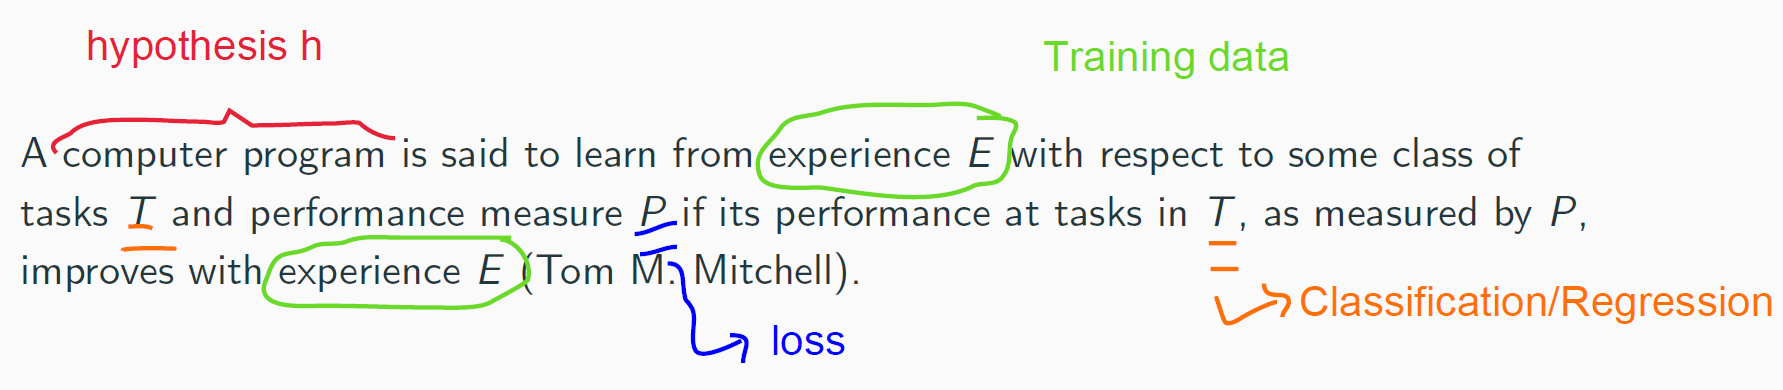
\includegraphics[width=\textwidth, clip]{images/setup_2}
\end{frame}

\begin{frame}{Back to the Supervised Learning Process}
	\centering
	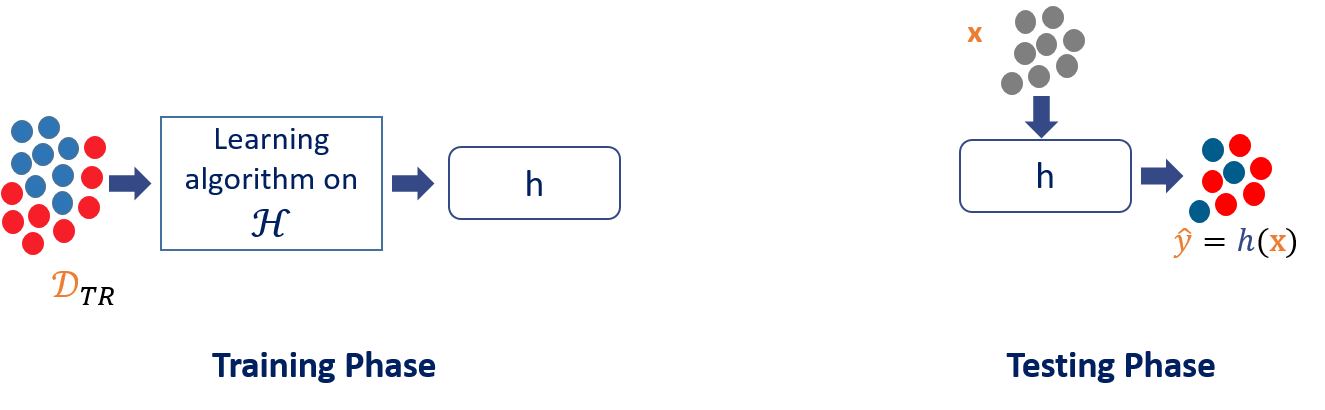
\includegraphics[width=\textwidth, clip]{images/supervised_process}
\end{frame}

\begin{frame}{The Learning Algorithm}
	Given a hypothesis class $\mathcal{H}$:
	\begin{enumerate}
		\item Train a model by minimizing the training loss:
			\begin{equation*}
			\hypothesis^* = \argmin{\hypothesis \in \mathcal{H}} \dfrac{1}{|\trainset_{TR}|}\sum_{(\boldx,\smally) \in \trainset_{TR}} \mathit{l}(\smally, \hypothesis(\boldx))
		\end{equation*}
		\item Evaluate the testing loss of the model:
		\begin{equation*}
			\epsilon_{TEST} = \dfrac{1}{|\trainset_{TEST}|}\sum_{(\boldx,\smally) \in \trainset_{TEST}} \mathit{l}(\smally, \hypothesis(\boldx))
		\end{equation*}
	\end{enumerate}
	\alert{Question:} As $|\trainset_{TEST}| \rightarrow \infty$, $\epsilon_{TEST} \rightarrow \epsilon$, why?

\end{frame}
\section{Wrap-Up}
\begin{frame}{Recap}
	\begin{itemize}
		\item We introduced the basic terminology used in supervised learning
		\item We formalized the supervised learning setup 
	\end{itemize}
\end{frame}

\begin{frame}{Key Concepts}
	\begin{itemize}
		\item Feature vector, attributes, input
		\item Label, target output
		\item Classification \& regression
		\item Hypothesis class
		\item Loss function
		\item Generalization
		\item Overfitting
		\item Data splits
		\item Training, validation and testing data
		\item No Free Lunch [\href{https://en.wikipedia.org/wiki/No_free_lunch_theorem}{link}]
	\end{itemize}
\end{frame}

	
\begin{frame}[t,standout]
	\Large
	Any questions?
\end{frame}

%\begin{frame}{Further Reading and Useful Material}
%	
%	\begin{table}
%		\begin{tabular}{|l | l | }
%			\hline
%			\multicolumn{1}{|c|}{\textbf{Source}} & \multicolumn{1}{c|}{\textbf{Notes}} \\
%			\hline
%			Samuel Checker's Player &	\href{https://link.springer.com/referenceworkentry/10.1007\%2F978-0-387-30164-8_740}{Encyclopedia of ML (link)} \\
%			Pattern Recognition and Machine Learning & Sec 1.5.5, Ch. 3 \\
%			\href{https://www.math.uwaterloo.ca/~hwolkowi/matrixcookbook.pdf}{The Matrix Cook Book} & \\
%			\href{http://vmls-book.stanford.edu/vmls.pdf}{Introduction to Linear Applied Linear Algebra}  & Part III – Least Squares\\
%			\hline
%		\end{tabular}
%	\end{table}
%	
%	
%\end{frame}

%\begin{frame}{Outlook}
%	\Large
%	The font size should be as large as possible
%	\begin{itemize}
%		\item \textit{Never smaller than the age of the oldest audience member}
%		\item Don't vary sizes to much, never within a slide
%		\item Stick to one font
%		\item Don't overuse formatting like bold, italics, alert, etc.
%	\end{itemize}
%	But you knew all that already...
%\end{frame}

\end{document}
